\documentclass{article}
\usepackage[utf8]{inputenc}
\usepackage[spanish]{babel}
\usepackage{listings}
\usepackage{graphicx}
\graphicspath{ {images/} }
\usepackage{cite}

\begin{document}

\begin{titlepage}
    \begin{center}
        \vspace*{1cm}
            
        \Huge
        \textbf{trabajo de investigacion}
        \vspace{0.5cm}
        \LARGE
        memoria en las computadoras
            
        \vspace{1.5cm}
            
        \textbf{Santiago Pereira Ramirez}
            
        \vfill
            
        \vspace{0.8cm}
            
        \Large
        Despartamento de Ingeniería Electrónica y Telecomunicaciones\\
        Universidad de Antioquia\\
        Medellín\\
        Septiembre de 2020
            
    \end{center}
\end{titlepage}

\tableofcontents

\section{Introduccion}
durante mucho tiempo se ha pensado que programar no mas que  escribir codigo, en gran parte no deberia ser asi,ni mucho menos pensado en la programacion.Para programar en un buen sentido de la palabra se debe de tener aspectos tales como la comprension y calidad del algoritmo que vamos a implementar,tener diferentes capacidades de comunicacion 
y formas de trabajar en equipo,asi como tener la disciplina y el empeño para realizar los diferentes trabajos asignados .Pero algo que es de suma importancia al programar es como sabemos manejar la memoria, como se compone y ademas como trabaja, algo que muchos dirian que nos es importante pero enrealidad es fundamental en el proceso, la memoria algo mucho mas que guardar.


\section{Sección de contenido} \label{contenido}
    \subsection{Qué es la memoria de un computador?}
    Podemos definir la memoria en un contexto general, podriamos decir que es el proceso por el cual la memoria tiene capacidad mental que posibilita a un sujeto registrar, conservar y evocar las experiencias\cite{hipocampo}, y si volvemos a leer de nuevo, podemos plantear que esta idea no se aleja mucho de la logica con la cual es programado un computador, aunque sin apegarnos a esto y ademas profundizando; la memoria en el computador tiene un proceso complejo y que para algunos tiene una ventaja sobre los humanos, alguna de estas como la velocidad, rapidez y eficiencia.
    
    Asi, la memoria en el computador cumple un papel fundamental para el buen funcionamiento del mismo.y aunque conceptualmente la memoria parezca sencilla,enrealidad presenta la mas amplia diversidad de arquitecturas, gamas y prestaciones\cite{academia}.
    Pero en contexto se puede decir que la memoria es la "parte" del computador que almacena la informacion que este maneja(datos y los programas para la ejecucion de estos procesada por los microprocesadores para la tareas asignadas por el usuario).\cite{academia}

    \begin{figure}[h]
    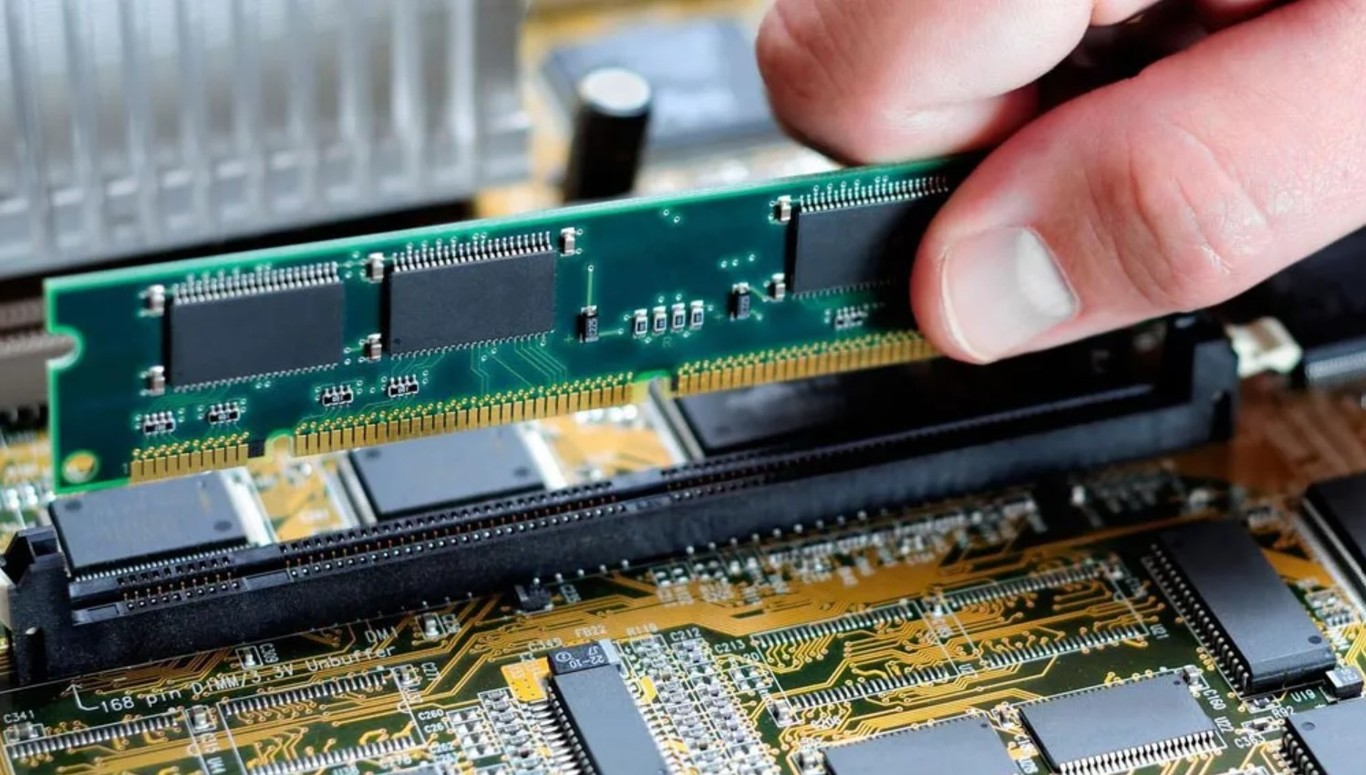
\includegraphics[width=6 cm]{imagenes/tipo_memoria.jpg}
    \centering
    \caption{foto memoria ram}
    \label{fig:tipo_memoria}
    \end{figure}

    Por otra parte podriamos decir que el termino de memoria es una taquigrafia(Técnica de escritura en la que se utilizan ciertos signos y abreviaturas especiales para poder transcribir todo lo que dice alguien a la misma velocidad a la que habla.) para la memoria fisica que se refiere a los chips que son capaces de llevar a cabo datos del computador \cite{monografias}.
    
    \subsection{Tipos de memoria}
    En las computadoras hay diferentes tipos de memoria, unas mas rapidaz que otras pero todas iguales de importantes y todas necesarias para el correcto funcionamiento, por ejemplo, hoy en dia los microprocesadores cada vez son mas eficientes y veloces, capaces de procesar miles de millones de ciclos por segundo,por ende son capaces de procesar miles de millones de bytes por segundo, por este motivo deben de tener dispositivos de almacenamiento temporal por que puedan seguir el trabajo ya que si no fuera asi se tendria que parar para cada informacion que llegue.\cite{profe}
    
        \subsubsection{memoria cache}
        la memoria cache es una memoria auxiliar, de gran velocidad y eficiencia. En ella se almacenan la copia de los archivos y datos con los que se accede con mayor frecuencia(ya sea en un computador o en un dispositivo movil),
        como dato curioso, su nombre es de origen frances que significa oculto o escondido, tiene la capacidad de operar de manera mucho mas rapida y eficiente, cada vez que se necesite de los datos almacenados en ella.\cite{academia1}
        
        Es importante decir que los datos menos utilizados en la memoria cache seran borrados de ella pero no de la memoria principal
        ubicada en los computadores entre la memoria RAM y la unidad central de procesamiento (GPU).
        La memoria cache consta de tres tipos los cuales son:
            
           
            -cache de nivel 1(L1): La memoria interna  esta integrada en el procesador y trabaja a la misma velocidad, y se divide en dos partes(una parte se encarga de almacenar las instrucciones y la otra los datos)
            
            
            -cache de nivel 2(L2) : Almacena datos y archivos , ls velocidad de esta cache comprada con la anterior es mucho menor y ademas no tiene divisiones en su estructura
            
           
            -cache de nivel 3(L3): es mucho mas rapida en cuanto al acceso de datos e instrucciones que no estan en L1 Y L2 , ademas la capacidad de respuesta es mucho mayor a la de la memoria principal sin contar que puede llegar hasta los 12 megabytes de almacenamiento.
        
        \subsubsection{La memoria RAM}
        La memoria RAM es el tipo de memoria mas importante que tiene el computador,en este tipo de memoria se puede acceder desde cualquier espacio , mo importa si dirreccion o la posicion. Las siglas RAM significan ( Random Access Memory o memoria de acceso aleatorio por su traduccion del ingles),es un gran componente y a medida que el computadoras tengan mas memoria RAM(Acequible en algunos casos)este no dependera tanto de la memoria virtual.
        
        --Tipos de memoria RAM:
            
            -DRAM(dynamic RAM): Por su traduccion al español RAM dinamica , es un tipo de memoria que envia señales llamadas RAS(señal de direccion de fila)hacia la fila donde se encuentran las celdas cuyo transistores se van a activar y permitir  pasar los electrones hacia los capacitores de las celdas, seguidamente se envian otro tipo de señales llamadas CAS(señales de direccion de columna) las cuales  rellenan con electrones los capacitores de las celdas que representan los bits 1.
            
            -SRAM (static RAM) : por su traduccion al español RAM estatica, en este "nuevo" tipo de memoria es diferente al tipo DRAM, esta compuesta por cuatro transistores y algunos circuitos, y gracias a esto permite ser mucho mas rapida que la memoria DRAM, aunque al ser mucho mas grande esto hara que tenga menor cantidad de celdas y asi menor capacidad de bits de almacenamiento.
            
            -SDRAM (Synchronous Dynamic RAM) : la RAM dinamica sincronica,funciona en sincronia con el microprocesador ,lo que significa que espera a la señal de reloj antes de responder,asi aceptando una orden de lectura antes  de haber procesado una orden de escritura(trabajar en paralelo).\cite{hardzone}
            
            \begin{figure}[h]
            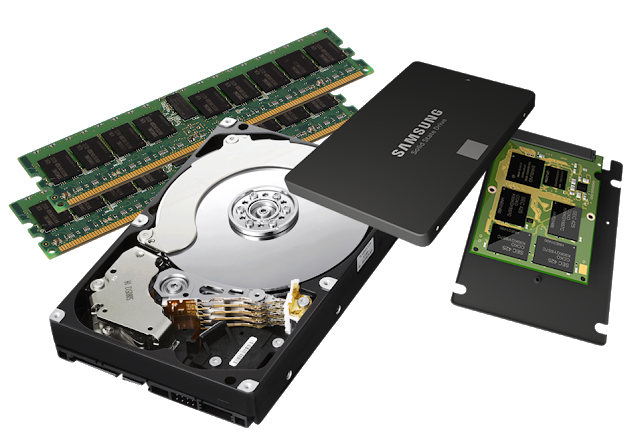
\includegraphics[width=6 cm]{imagenes/ram+hdd+ssd.png}
            \centering
            \caption{foto memoria RAM y el disco duro}
            \label{fig:ram+hdd+ssd}
            \end{figure}
            
        \subsubsection{La memoria virtual}
        La memoria virtual es una porcion del disco duro destinada a sostener temporalmente trozo de programas y datos que estan en ejecucion y utilizan espacio innecesario(si hay muy poca memoria RAM y a su vez el computador esta consumiendo mucha puede ocurrir la hiperpaginacion volviendolo muy lento).

        \subsubsection{Disco Duro}
        El disco duro es el tipo de memoria que guarda datos a largo plazo y ademas no se borran al apagar el PC, es el responsable de guardar el codigo del sistema operativo y los programas que dia a dia utilizamos,como parte esencial se debe de tener en cuenta que cada tipo de disco duro tiene su espacio y consumido en parte por el sistema operativo e instalaciones de respaldo.\cite{digitaltrends}
        
        \subsubsection{La memoria ROM}
        Es conocida como memoria de solo lectura(read only memory), este tipo de memoria utilizado en ordenadores y dispositivos electronicos solo permite la lectura de la informacion y no de su escritura;Independientemente  de la presencia o no de la fuente de energia. Ademas de esto  cuando se emplea en una computadora tiene como proposito tambien almacenar programas,datos fijos que se desea que sean inalterables y  almacenando tablas de constantes que no deberian estar sujetas a cambio.\cite{aca}
    
    \subsection{¿Como se gestiona la memoria en un computador?}
    La memoria se gestiona mediante algunos pasos, que podrian organizarce de la siguiente manera:
    
        \subsubsection{Reasignacion} El proceso empieza mediante la orden del usuario, que temporalmente quedara en un espacio en la memoria.\cite{wikipedia}
        
        \subsubsection{proteccion} Los procesos no pueden distinguir entre los procesos de memoria y otros tipos de procesos que no tienen permisos, para esto existe la proteccion de la memoria que evita el codigo malicioso que pueda interferir en los procesos, tambien es otro metodo para controlar el uso de memoria de una PC  y cuenta con diferentes metodos como los son(segmentacion,paginas,llaves de proteccion, segmentacion simulada y direccionamiento basado en la capacidad.)\cite{wiki}
        
    
        \subsubsection{administrador de memoria}El microprocesador buscara la orden y la ejecutara, seguido la orden se eliminara del procesador y ademas del espacio de memoria.
    
        \subsubsection{Tecnicas de administracion de memorias(asignacion contigua)}   Ya hecho lo anterior el procesador manda una orden al controlador el cual esta ubicado en la motherboard o tarjeta madre.El controlador toma el programa o la orden del disco duro y la desplaza hacia un espacio de memoria para trabajar sobre él.Ya que no hay tanta capacidad de informacion el microprocesador trabaja con la memoria, a tal caso trabaja por porciones del programa, asi llevando y trayendo del procesador hacia la memoria,ahora se da la orden de traer un documento compatible para trabajar con el programa(mismos pasos explicados anteriormente )  y carga en un espacio de memoria.El microprocesador se da cuenta de que hay una instruccion en un espacio de la memoria, la busca, la coge y la procesa, elimina el espacio en memoria ya que es innecesario y nuevamente le da una instruccion al controlador para que tome el archivo y lo ponga en un espacio vacio de la memoria.\cite{profe}
        
        Llegados a este punto el micropocesador utiliza los recursos del programa para trabajar sobre el documento, al querer guardar el documento el usuario mediante el mouse manda una instruccion hacia la memoria, acto seguido el microprocesador resive la instruccion y se dara la tarea de ir,tomarla ,leerla y eliminar la instruccion del espacio de memoria,despues se envia  una orden al controlador(guardar el documento en el cual trabajamos, sobreescribirlo en el disco duro con el mismo nombre); ya hecho el trabajo el usuario dara la orden de cerrar el programa que llegara al controlador de la motherboard y viajara por el bus de datos( la información, instrucciones y datos viajan de un dispositivo a otro por el bus de datos,circuitos impresos de cobre que se ven sobre la placa madre o
        motherboard si se abre el computador.)hasta llegar  a la memoria del computador.\cite{profe}
        
        \subsubsection{Ordenes finales} Ahora el microprocesador da  un aviso de orden, la pasa a buscar, leer y procesar(lo cual no es mas que quitar tanto el documento como el programa del espacio de memoria en el cual estaban.)
        

    \subsection{Qué hace que una memoria sea más rápida que otra y porque esto es importante?}
    
    Cuando hablamos de rapidez tendemos a igualarla con la velocidad, terminos que parecen ser iguales pero que en realidad tienen ciertas diferenciaciones. Asi mismo la rapidez de  una memoria podria decirse que se compone de la latencia(eficiencia) y la frecuencia(velocidad).Pero en un campo mas amplio que significa cada uno de ellas?.
    
    \subsubsection{Latencia} La latencia es el tiempo que transcurre entre una peticion y respuesta,para profundizar mas La latencia CAS mide el número de ciclos de reloj que pasan desde que se realiza una petición para leer un dato hasta que dicha información está disponible.Pero enrealidad el tiempo de latencia no sera el total que se calcule ya que entra algo que influye mucho y que reduce el tiempo en que se hace un ciclo que es la frecuencia.\cite{profesional}
    
    \subsubsection{Frecuencia} Es la que indica la velocida a la que trabaja la memoria,mas aun el numero de frecuencia indica cuantos datos puede manejar por segundo, entonces mientras mas ciclos sobre segundos mas cantidad de datos se podra almacenar y leer, asi beneficiando al usuario ya que sera todo mas fluido(como ejemplo podemos plantear que una memoria RAM tiene 3200 MHz, por ende esta ejecutará 3.200 millones de ciclos por segundo).\cite{computerhoy}
    
    dos formulas bastante faciles para calcular el rendimiento  serian: 
    
    (Latencia/Frecuencia) x 2 x 1024
    
    un ejemplo para esta formula seria: una memoria que tiene 8 de latencia o timing y una frecuencia de 2.133 MHz daria un rendieminto de 9,60 nanosegundos[ (10/2.133) x 2 x 1024= 9,60 ns].
    
    En conclucion una memoria es mas rapida que otra gracias a una adecuada latencia (ya que nos permitira menos esperas en las entrasdas de datos) y una buena frecuencia, importante en todos los casos ya que nos dara eficiencia, fluidez y un desarrollo optimo.

\begin{lstlisting}

\end{lstlisting}

\section{Conclusión} \label{conclulsion}
La memoria no solo es hardware que solo utilizamos para guardar y obtener datos, va mucho mas alla. Es indispensable saber el funcionamiento de cada una, que las componen y su comportamiento, asi al programar o utilizar los programas, podremos programar sistemas mas optimos o usarlos de la mejor manera, ver de otra forma la manera en que vemos la estructura de la maquina y la manera en que trabajamos; entender y sensibilizar nuestro pensamiento respecto a lo que manejamos es lo importante en el aprendizaje y nuestro oficio.

\bibliographystyle{IEEEtran}
\bibliography{references}

\end{document}
